
%-------------------------------------------------------------------------------
%                             ADDITIONAL PACKAGES
%-------------------------------------------------------------------------------
\documentclass[
	a4paper,
%	showframes,
%	vline=2.2em,
%	maincolor=cvgreen,
%	sectioncolor=red,
%	subsectioncolor=orange,
%	itemtextcolor=black!80,
%	sidebarwidth=0.4\paperwidth,
%	topbottommargin=0.03\paperheight,
%	leftrightmargin=20pt,
%	profilepicsize=4.5cm,
%	profilepicborderwidth=3.5pt,
%	profilepicstyle=profilecircle,
%	profilepiczoom=1.0,
%	profilepicxshift=0mm,
%	profilepicyshift=0mm,
% profilepicrounding=1.0cm,
]{fortysecondscv}

% define divider and cvdivider command: dashed gray line separator
% attention: import colortbl befor arydshln
\usepackage{colortbl}
\usepackage{arydshln}
\RequirePackage{dashrule}
\colorlet{body}{black!80!white}
\newcommand{\cvdivider}{\arrayrulecolor{body!30}\hdashline}
\newcommand{\profiledivider}{\textcolor{body!30}{\hdashrule{\linewidth}{0.6pt}{0.5ex}}\\}
%\newcommand{\divider}{\textcolor{body!30}{\hdashrule{\linewidth}{0.6pt}{0.5ex}}}

% Portuguese package (used in signature date)
%\usepackage[portuguese]{babel}

% package used to wrap text around a figure
\usepackage{wrapfig}

% provides blind text useful for test purposes
\usepackage{blindtext}

\usepackage{amsmath}
\usepackage{multirow}
\usepackage{makecell}
\usepackage{array}

% include fonts
\pdfmapfile{=ClearSans.map}
\pdfmapfile{=fontawesome.map}

% include and use scalable cm-super fonts
\usepackage[T1]{fontenc}
\usepackage{lmodern}

% improve word spacing and hyphenation
\usepackage{microtype}
\usepackage{ragged2e}

% provides blind text useful for test purposes
\usepackage{blindtext}

\usepackage{amsmath}

% include fonts
\pdfmapfile{=ClearSans.map}
\pdfmapfile{=fontawesome.map}

% include and use scalable cm-super fonts
\usepackage[T1]{fontenc}
\usepackage{lmodern}

% improve word spacing and hyphenation
\usepackage{microtype}
\usepackage{ragged2e}

% take care of proper font encoding
\ifxetexorluatex
	\usepackage{fontspec}
	\defaultfontfeatures{Ligatures=TeX}
%	\newfontfamily\headingfont[Path = fonts/]{segoeuib.ttf} % local font
\else
	\usepackage[utf8]{inputenc}
	\usepackage[T1]{fontenc}
%	\usepackage[sfdefault]{noto} % use noto google font
\fi

% enable mathematical syntax for some symbols like \varnothing
\usepackage{amssymb}

% bubble diagram configuration
%\usepackage{smartdiagram}
%\smartdiagramset{
%	% default font size is \large, so adjust to harmonize with sidebar layout
%	bubble center node font = \footnotesize,
%	bubble node font = \footnotesize,
%	% default: 4cm/2.5cm; make minimum diameter relative to sidebar size
%	bubble center node size = 0.4\sidebartextwidth,
%	bubble node size = 0.25\sidebartextwidth,
%	distance center/other bubbles = 1.5em,
%	% set center bubble color
%	bubble center node color = maincolor!70,
%	% define the list of colors usable in the diagram
%	set color list = {maincolor!10, maincolor!40,
%	maincolor!20, maincolor!60, maincolor!35},
%	% sets the opacity at which the bubbles are shown
%	bubble fill opacity = 0.8,
%}


%-------------------------------------------------------------------------------
%                            PERSONAL INFORMATION
%-------------------------------------------------------------------------------
%% mandatory information
% your name
\cvname{Rafael Claro Ito}
% job title/career
\cvjobtitle{
    Electrical Engineer\\[0.2em]
    HW \& SW Developer\\[0.2em]
    Data Scientist
}






%\graphicspath{{../figures/whoami/}}
%\newcommand{\whoamiemail}{\cvicon{\includegraphics[align=c, width=1.0em]{email}}}
%\whoamiemail




%% optional information
% profile picture
\cvprofilepic{../figures/profile.jpeg}

% NOTE: ordering in sidebar will mimic the following order
% date of birth
\cvbirthday{03/02/1992}
% short address/location, use \newline if more than 1 line is required
%\cvaddressone{Rua Gilberto Pattaro, 150 $\cdot$ Campinas/SP, Brazil}
\cvaddressone{Rua Gilberto Pattaro, 150 $\boldsymbol{\cdot}$ 13084-375}
\cvaddresstwo{Campinas, SP $\boldsymbol{\cdot}$ Brazil}
% phone number
\cvphone{+55 19 98810-2615}
% personal website
%\cvsite{https://pandascience.net}
% email address
\cvmail{ito.rafael@gmail.com}
% pgp key
%\cvkey{4096R/FF00FF00}{0xAABBCCDDFF00FF00}
% any other custom entry
%\cvcustomdata{\faFlag}{Chinese}

%\cvline{\hline}
%\cvline{}

\cvlinkedin{https://www.linkedin.com/in/itorafael/}{linkedin.com/in/itorafael}
\cvgithub{https://github.com/ito-rafael/}{github.com/ito-rafael}
\cvfacebook{https://www.facebook.com/ito.rafael92}{facebook.com/ito.rafael92}
\cvskype{}{ito.rafael92}

%-------------------------------------------------------------------------------
%                              SIDEBAR 1st PAGE
%-------------------------------------------------------------------------------
% add more profile sections to sidebar on first page
\addtofrontsidebar{

%    %===============
%    % SOCIAL NETWORK
%    %===============
%	% social network accounts incl. proper hyperlinks
%	\profilesection{Social Network}
%		\begin{icontable}{2.5em}{1em}
%%			\social{\aiOverleafSquare}
%				%{https://de.overleaf.com/latex/templates/forty-seconds-cv/pztcktmyngsk}
%			\social{\faLinkedin}
%                {https://www.linkedin.com/in/itorafael/}
%                {linkedin.com/in/itorafael}
%				%{LinkedIn}
%			\social{\faGithub}
%				{https://github.com/ito-rafael/}
%				{github.com/ito-rafael}
%				%{ito-rafael}
%            \social{\faFacebookSquare}
%                {https://www.facebook.com/ito.rafael92}
%                {facebook.com/ito.rafael92}
%            \social{\faSkype}
%                {}
%                {ito.rafael92}
%		\end{icontable}

    %===============
    % LANGUAGES
    %===============
	% include gosquare national flags from https://github.com/gosquared/flags;
	% naming according to ISO 3166-1 alpha-2 country codes
    \graphicspath{{../figures/languages/}}

	\profilesection{Languages}
		\pointskill{\flag{en-US}}{English}{5}
		\pointskill{\flag{pt-BR}}{Portuguese}{5}
	    \pointskill{\flag{it-IT}}{Italian}{4}
    	\pointskill{\flag{fr-FR}}{French}{2}
    	\pointskill{\flag{es-ES}}{Spanish}{2}
    	\pointskill{\flag{jp-JP}}{Japanese}{1}

    %===============
    % AWARDS
    %===============
    \profilesection{Awards}
        % insert path for awards icon
        \graphicspath{{../figures/awards/}}
        % define new commands for awars icon
        \newcommand{\goldenmedal}{\cvicon{
\includegraphics[align=c, width=1.0em]{medal_golden_red}}}
        \newcommand{\silvermedal}{\cvicon{
\includegraphics[align=c, width=1.0em]{medal_silver_blue}}}
        \newcommand{\certificate}{\cvicon{
\includegraphics[align=c, width=1.0em]{merit}}}
        \newcommand{\certificatetwo}{\cvicon{
\includegraphics[align=c, width=1.0em]{merit_2}}}
        
        \skill{\goldenmedal}{2009 6th place at OSA}
		\skill{\silvermedal}{2009 Silver Medal at OBMEP}
		\skill{\silvermedal}{2008 Silver Medal at OBMEP}
		\skill{\certificatetwo}{2008 Certificate of Merit at OMU}
		\skill{\certificate}{2007 Honorable Mention at OBMEP}
		\skill{\certificate}{2006 Honorable Mention at OBMEP}
        %--------------------------------------------------------
        \profiledivider
        {\scriptsize
            OBMEP: Brazilian Public Schools Mathematics Olympiad\\
            OSA: UNICAMP Physics Olympiad\\
            OMU: UNICAMP Mathematics Olympiad
            \par
        }

    %===============
    % REFERENCES
    %===============
    \profilesection{References}
    	\cvreference
            %{\faBalanceScale}
            {\textcolor{iconcolor}{\hskip 0.19em \large\faBalanceScale} \hskip 0.1em
            \textbf{João da Silva}
            \smallskip\newline\medskip
            %\footnotesize{Head of blah}\newline
            Head of blah\newline
            $\boldsymbol{\cdot}$ \textbf{Relação:} ex-boss\newline
            $\boldsymbol{\cdot}$ \textbf{contato:} joao.silva@gmail.com}
        %---------------------------------------
        \profiledivider
        %---------------------------------------
    	\cvreference
        {\vskip 0.7ex \textcolor{iconcolor}{\hskip 0.19em \large\faBriefcase} \hskip 0.1em
            \textbf{Fulano Beltrano}
            \smallskip\newline\medskip
            %\footnotesize{Professor at Unicamp} \newline
            Professor at Unicamp\newline
            $\boldsymbol{\cdot}$ \textbf{Relação:} ex-professor\newline
            $\boldsymbol{\cdot}$ \textbf{contato:} fulanobeltra@gmail.com}


%	\profilesection{Hard Skills}
%		\skill{\faBalanceScale}{Sleeping almost all day}
%		\skill{\faSitemap}{Eating a lot bamboo sprouts}
%		\skill{\faGraduationCap}{Relaxing rest of the day}

%	\profilesection{Soft Skills}
%		\pointskill{\faHome}{Looking Cute}{4}[4]
%			\skill[1.8em]{\faCompress}{No need to specify further}
%		\pointskill{\faChild}{Chillin' hard}{3}[4]
%			\skill[1.8em]{\faCompress}{On a tree}
%			\skill[1.8em]{\faCompress}{On the grass}

}


%-------------------------------------------------------------------------------
%                              SIDEBAR 2nd PAGE
%-------------------------------------------------------------------------------
\addtobacksidebar{
	\profilesection{About Me}
	\aboutme{
		The giant panda is a terrestrial animal and primarily spends its life
		roaming and feeding in the bamboo forests of the Qinling Mountains and in
		the hilly province of Sichuan.
	}

	\profilesection{Diagrams}
	\chartlabel{Bubble Diagram}
	\begin{figure}\centering
		\smartdiagram[bubble diagram]{
			\textcolor{white}{\textbf{Being a}} \\
			\textcolor{white}{\textbf{Panda}}, % center bubble
			\textcolor{black!90}{Eating},
			\textcolor{black!90}{Sleeping},
			\textcolor{black!90}{Rolling},
			\textcolor{black!90}{Playing},
			\textcolor{black!90}{Chilling}
		}
	\end{figure}

	\chartlabel{Wheel Chart}

	\wheelchart{4em}{2em}{%
	20/3em/maincolor!50/Chill,
	15/3em/maincolor!15/Play,
	30/4em/maincolor!40/Sleep,
	20/3em/maincolor!20/Eat
	}

	\profilesection{Barskills}
	\barskill{\faSkyatlas}{Wearing asian rice hats}{60}
	\barskill{\faImage}{Playing Chess}{30}
	\barskill{\faMusic}{Playing the bamboo flute}{50}

	\profilesection{Memberships}
	\begin{memberships}
        \membership[4em]{../figures/logo.png}{PandaScience.net}
        \membership[4em]{../figures/logo.png}{Some long text spanning over more than
			only one line}
            \membership[4em]{../figures/logo.png}{\rule{\linewidth}{1pt}}
	\end{memberships}
}


%-------------------------------------------------------------------------------
%                         TABLE ENTRIES RIGHT COLUMN
%-------------------------------------------------------------------------------
\begin{document}

\makefrontsidebar

%=======================================
\cvsection{Working Experience}
%=======================================
% change arraystretch (distance between items):
%\begin{cvtable}[<arraystretch>=1]
%\begin{cvtable}[1.5]
\graphicspath{{../figures/work/}}
\newcolumntype{L}{>{\centering\arraybackslash}m{5.5cm}}
%	%\cvitem
    \cvevent
        {Technological Development Analyst}
        {CNPEM/LNLS}
        {Jan 2016 -- current}
        {Campinas/SP}
        {\hspace{2mm}
\includegraphics[height=0.07\textwidth]{CNPEM}}
        {Blah}
    %---------------------------------------
    \\\profiledivider
    %---------------------------------------
	%\cvitem{Jan 2016 Jul 2016}{Teaching Assistant}{University of Campinas}{bla alkdjasjd asdjasd asiod asoidj asoid jasdj asoidj as djaskldjaslkd jalsdjlasjda daskl djalskdlajs ldasj dlkasj daskldj alsjdasld lasdasd aslj dlasdj asl djlas ldajl dasjd asl dlasjd\medskip}
	%\cvitem
    \cvevent
        {Teaching Assistant}
        {University of Campinas}
        {Jan 2016 -- Jul 2016}
        {Campinas/SP}
        {\hspace{2mm}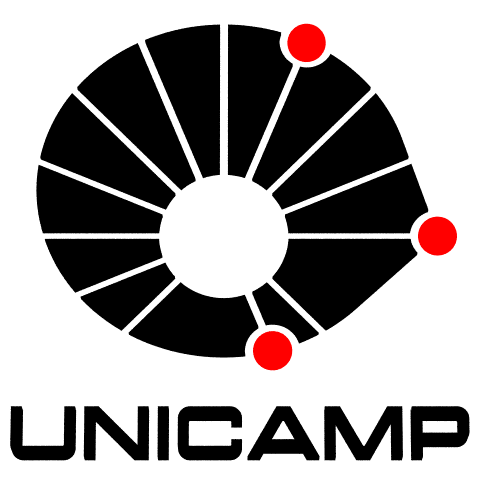
\includegraphics[height=0.07\textwidth]{Unicamp}}
        {\blindtext}
    %---------------------------------------
    \\\profiledivider
    %---------------------------------------
	%\cvitem
    \cvevent
        {Scientific Research}
        {Queen Mary University of London}
        {Jun 2015 -- Sep 2015}
        {London}
        {\hspace{2mm}
\includegraphics[height=0.07\textwidth]{QMUL}}
        {blabljdbjsdl bksdjblsdblds bjsd bkljsd blksjd blksdj blsd jblsd blksdjb lksdj blkds jblskd bjsdbjksdl bjlsdjblsd jblsdb sdlk bjlds jbsdkl bdsjl bkldsj blsd lbj s dblsdb sd kbj sdlkbjdskl bjdskl jbldsj b}
    %---------------------------------------
    \\\profiledivider
    %---------------------------------------
	%\cvitem{Jan 2010 Jun 2010}{Electronics intern}{CPqD - Telecommunications Research and Development Centre}{bla\medskip}
	%\cvitem
    \cvevent
        {Electronics intern}
        {CPqD - Telecommunications Research and Development Centre}
        {Jan 2010 -- Jun 2010}
        {Campinas/SP}
        {\hspace{2mm}
\includegraphics[height=0.07\textwidth]{CPqD}}
        {bla}
    %---------------------------------------
    \\\profiledivider
    %---------------------------------------
    %\cvitem
    \cvevent
        {Teaching Assistant}
        {Technical College of Campinas}
        {Jan 2009 -- Dec 2009}
        {Campinas/SP}
        {\hspace{2mm}
\includegraphics[height=0.07\textwidth]{Cotuca}}
        {bla}
    %---------------------------------------

%=======================================
\cvsection{Education}
%=======================================
%\cvsubsection{Postgraduate Training}
\graphicspath{{../figures/education/}}
%\begin{cvtable}[1.5]
    \cvevent
        {Graduate}
        {University of Campinas}
        {Jan 2017 -- current}
        {Campinas/SP}
        {\hspace{2mm}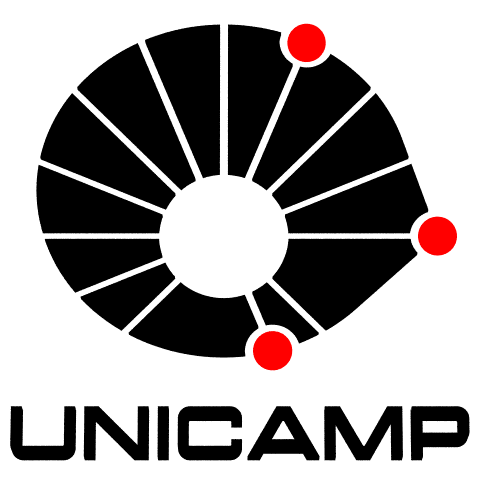
\includegraphics[height=0.07\textwidth]{Unicamp}}
        {Part-time Masters degree.}
    %---------------------------------------
    \\\profiledivider
    %---------------------------------------
	\cvevent
        {Undergraduate}
        {University of Campinas}
        {Jan 2011 -- Dec 2016}
        {Campinas/SP}
        {\hspace{2mm}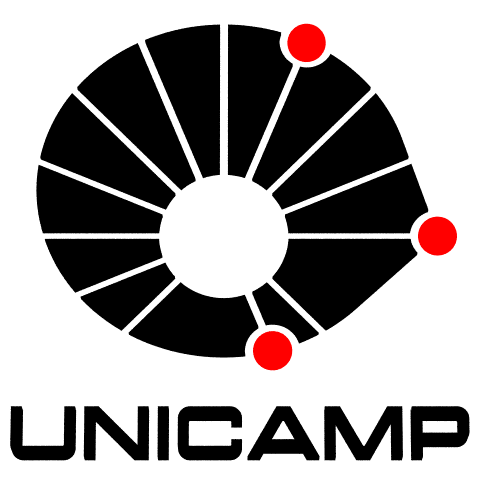
\includegraphics[height=0.07\textwidth]{Unicamp}}
        {Bla}
    %---------------------------------------
    \\\profiledivider
    %---------------------------------------
    \cvevent
        {Undergraduate (Student Exchange Program)}
        {Queen Mary University of London}
        {Sep 2014 -- Aug 2015}
        {London}
        {\hspace{2mm}
\includegraphics[height=0.07\textwidth]{QMUL}}
        {Studies sponsored by the Brazilian government due to academic merit. Science without Borders (SwB) student exchange program.}
    %---------------------------------------
    \\\profiledivider
    %---------------------------------------
	\cvevent
        {Further Education}
        {Technical College of Campinas - UNICAMP}
        {Jan 2007 -- Jul 2010}
        {Campinas/SP}
        {\hspace{2mm}
\includegraphics[height=0.07\textwidth]{Cotuca}}
        {Selected to work as a Teaching Assistant of the technical course.}
    %---------------------------------------

%\cvsubsection{Study}
%\begin{cvtable}[1.5]
%	\cvitem{2006 -- 2008}{Master Studies Panda Science}{Panda Academy}
%		{Focus: Advanced rice hat studies and nouveau rain-reflecting cover
%		materials.}
%	\cvitem{}{Master Theses ($\varnothing\,	1,0$)}{Asian Rice Hat Institute}
%		{Impact on solar radiation onto rice hat cover materials with special
%		attention to water resistance.}
%	\cvitem{2003 -- 2006}{Bachelor Studies PandaScience}{Panda Academy}
%		{Focus: Bamboo morphology and its usage in different craftmanships.}
%	\cvitem{}{Bachelor Theses ($\varnothing\,	1,0$)}{Bamboo Institute}
%		{The bambo flute: An underestimated instrument in orchestras?}
%\end{cvtable}

\cvsection{Publications}
\begin{cvtable}
	\cvpubitem
        {Cooking: 100 recipes for lazy Pandas}
        {Me and My Panda Friends}
		{Panda's Culinary World}
        {2010}
    %---------------------------------------
	\cvpubitem
        {Pandastasia}
        {Still Me}
        {Bamboo Books Assoc.}
        {2005}
\end{cvtable}


%=======================================
\cvsection{Awards}
%=======================================
\begin{cvtable}
	\cvitem{2010 -- now}{Panda of the Year}{Panda World Forum}{}
	\cvitem{2005 -- now}{Face of World Wide Fund for Nature}{WWF}{}
	\cvitem{2000}{Winner of Bamboo Sprouts Eating Contest}{Bamboo Society}{}
\end{cvtable}


%=======================================
\cvsection{Extra-Curricular Activities}
%=======================================
\begin{cvtable}
	\cvitemshort{Relaxing}{Master the fine art of relaxing everywhere}
	\cvitemshort{Music}{Playing the bamboo flute in the 1st Panda Orchestra}
	\cvitemshort{Education}{Teaching young pandas to be more panda-like}
\end{cvtable}


\newpage
%\makebacksidebar


\cvsection{section}
\cvsubsection{Subsection}
\begin{cvtable}
	\cvitem{<dates>}{<cv-item title>}{<location>}{<optional: description>}
\end{cvtable}

\cvsection{cvitem}
\cvsubsection{Multi-line with longer description}
\begin{cvtable}
	\cvitem{date}{Description}{location}{Some longer and more detailed
		description, that takes two lines of space instead of only one.}
	\cvitem{date}{Description}{location}{Some longer and more detailed
		description, that takes two lines of space instead of only one.}
	\cvitem{date}{Description}{location}{Some longer and more detailed
		description, that takes two lines of space instead of only one.}
\end{cvtable}

\cvsubsection{One-line without description}
\begin{cvtable}
	\cvitem{Award}{One-line description}{Sponsor}{}
	\cvitem{Award}{One-line description}{Sponsor}{}
	\cvitem{Award}{One-line description}{Sponsor}{}
\end{cvtable}

\cvsection{cvitemshort}
\cvsubsection{One-line}
\begin{cvtable}
	\cvitemshort{Key}{Some further description}
	\cvitemshort{Key}{Some further description}
	\cvitemshort{Key}{Some further description}
\end{cvtable}

\cvsubsection{Multi-line with longer description}
\begin{cvtable}
	\cvitemshort{Key}{Some further description. Can fill even more than
		only one single line while still keeping the correct indendation level.}
	\cvitemshort{Key}{Some further description. Can fill even more than
		only one single line while still keeping the correct indendation level.}
	\cvitemshort{Key}{Some further description. Can fill even more than
		only one single line while still keeping the correct indendation level.}
\end{cvtable}

\cvsection{cvpubitem}
\begin{cvtable}
	\cvpubitem{Publication title}{Authors}{Journal}{Year}
	\cvpubitem{Publication title}{Authors}{Journal}{Year}
	\cvpubitem{Publication title that is spanning over multiple lines and still
		does not look too bad}{Authors}{Journal}{Year}
\end{cvtable}

\cvsignature

\end{document}
